%%% Springer Nature Journal Template (sn-jnl.cls)
%%% Converted from LNCS (llncs) format

\documentclass[pdflatex,sn-mathphys-num]{sn-jnl}

%%% Standard Packages
\usepackage{graphicx}
\usepackage{multirow}
\usepackage{amsmath,amssymb,amsfonts}
\usepackage{amsthm}
\usepackage{mathrsfs}
\usepackage{xcolor}
\usepackage{textcomp}
\usepackage{booktabs}
\usepackage{array}
\usepackage{url}
\usepackage{caption}
\geometry{top=24mm,bottom=24mm,left=24mm,right=24mm}

\raggedbottom

\renewcommand\topfraction{.95}
\renewcommand\bottomfraction{.95}
\renewcommand\textfraction{.05}
\renewcommand\floatpagefraction{.90}
\setlength{\floatsep}{8pt plus 2pt minus 2pt}
\setlength{\textfloatsep}{10pt plus 2pt minus 2pt}
\setlength{\intextsep}{8pt plus 2pt minus 2pt}
\setlength{\abovecaptionskip}{4pt}
\setlength{\belowcaptionskip}{4pt}

\setlength{\floatsep}{6pt plus 2pt minus 2pt}
\setlength{\textfloatsep}{8pt plus 2pt minus 2pt}
\setlength{\intextsep}{6pt plus 2pt minus 2pt}
\setlength{\abovecaptionskip}{3pt}
\setlength{\belowcaptionskip}{3pt}


\begin{document}

\title[Comparative US AQI Time Series Forecasting in California]{Comparative US AQI Time Series Forecasting in California with Extreme-Event and Climate-Context Evaluation}

\author*[1]{\fnm{Nguyen Anh Minh} \sur{Ta}}\email{taminh123xt@gmail.com}
\author[1]{\fnm{Thu} \sur{Le}}\email{thulvm@fpt.edu.vn}
\author[1]{\fnm{Quoc Sang} \sur{Trinh}}\email{trinhquocsang1@gmail.com}
\author[1]{\fnm{Nhat-Tung} \sur{Le}}\email{tungln4@fpt.edu.vn}

\affil*[1]{\orgname{FPT University}, \orgaddress{\city{Ho Chi Minh City}, \country{Vietnam}}}

\abstract{California hourly Air Quality Index (AQI) dynamics exhibit strong short-term autocorrelation alongside sudden volatility during wildfire seasons. Standard annual averages mask model vulnerabilities during severe pollution spikes. We benchmark five tabular regressors and two baselines across 181,122 hourly records (2018--2025). A chronological split reserves the smoke-heavy 2020 season for validation, evaluating nowcasting and 24-hour forecasting on the 2025 holdout set. XGBoost achieves top $R^2$ scores of 0.8711 (short-term) and 0.4648 (24-hour). Scenario slicing shows machine learning performance degrades sharply during upper-tail extremes, where persistence baselines match or beat complex models. Feature ablations show engineered vapor pressure deficit (VPD) and spatial lags offer marginal standalone accuracy gains. We operationalize these findings in a real-time early warning dashboard.}

\keywords{US AQI forecasting, PM2.5, California, time-series regression, climate-context evaluation, vapor pressure deficit, spatial lag, XGBoost, extreme-event analysis}

\maketitle

\section{Introduction}\label{sec:introduction}
Accurate air quality forecasts guide public health warnings and environmental regulation. In California, complex interactions between urban emissions, marine air masses, terrain, and wildfire smoke make hourly AQI prediction difficult. Models performing well under typical conditions often fail during severe pollution episodes. Random data splits also introduce severe temporal leakage due to autocorrelation.

This study benchmarks tabular machine learning models on a multi-city California dataset, addressing two main questions. First, how do gradient boosting and linear models perform when shifting from short-term nowcasting to a strict 24-hour horizon? Second, do these models maintain reliability when evaluated on isolated extreme events rather than full-year averages?

We present four key contributions. First, we construct a 181,122-record hourly panel combining EPA AQS observations and Open-Meteo weather fields \cite{epa_aqs,epa_aqs_api}. Second, we enforce a climate-aware temporal split reserving 2020 for wildfire-context validation and 2025 for final testing. Third, we test physically motivated features, including vapor pressure deficit (VPD) and cross-station spatial lags. Fourth, we combine global metrics with scenario stress tests and deploy an interactive alert dashboard.

\section{Related Work}\label{sec:related-work}
Air quality forecasting traditionally relied on statistical autoregressive models. While interpretable, linear methods struggle with complex weather interactions. Tabular machine learning provides flexible alternatives. Random Forest offers robust bagging-based ensemble predictions \cite{breiman2001random}, whereas gradient-boosted decision trees—XGBoost, LightGBM, and CatBoost—capture non-linear environmental thresholds \cite{chen2016xgboost,ke2017lightgbm,prokhorenkova2018catboost}. Spatial lag features from adjacent monitoring sites also enhance regional inference \cite{zheng2013uair}.

For wildfire PM2.5 estimation, Vu et al.\ \cite{vu2022geostationary} modeled the 2018 California Camp Fire using a weighted Random Forest. Merging AQS monitors, PurpleAir sensors, GOES-16 satellite data, and HRRR meteorology with SMOTE oversampling, they achieved an out-of-bag $R^2$ of 0.92 and a temporal cross-validation $R^2$ of 0.85. Their results show the value of combining ground and satellite data during extreme smoke events. We build on their work by incorporating engineered dryness metrics and spatial lags into a multi-year AQI forecasting panel.

Validation design remains critical. Random cross-validation leaks temporal information across adjacent hours, inflating performance \cite{bergmeir2018note,roberts2017crossvalidation}. We prevent this by enforcing strict chronological splits and isolating the extreme 2020 wildfire season for validation.

\section{Dataset and Exploratory Analysis}\label{sec:dataset}
\subsection{Study Area and Data Sources}\label{subsec:study-area}
The dataset covers Fresno, Los Angeles, and San Jose, pairing EPA AQS monitoring logs with Open-Meteo meteorological and AQI variables. The target variable, \texttt{target\_aqi}, is a PM2.5-derived AQI proxy. Raw PM2.5 and PM10 proxy features are removed to prevent direct target leakage.

\begin{figure}[htbp]
    \centering
    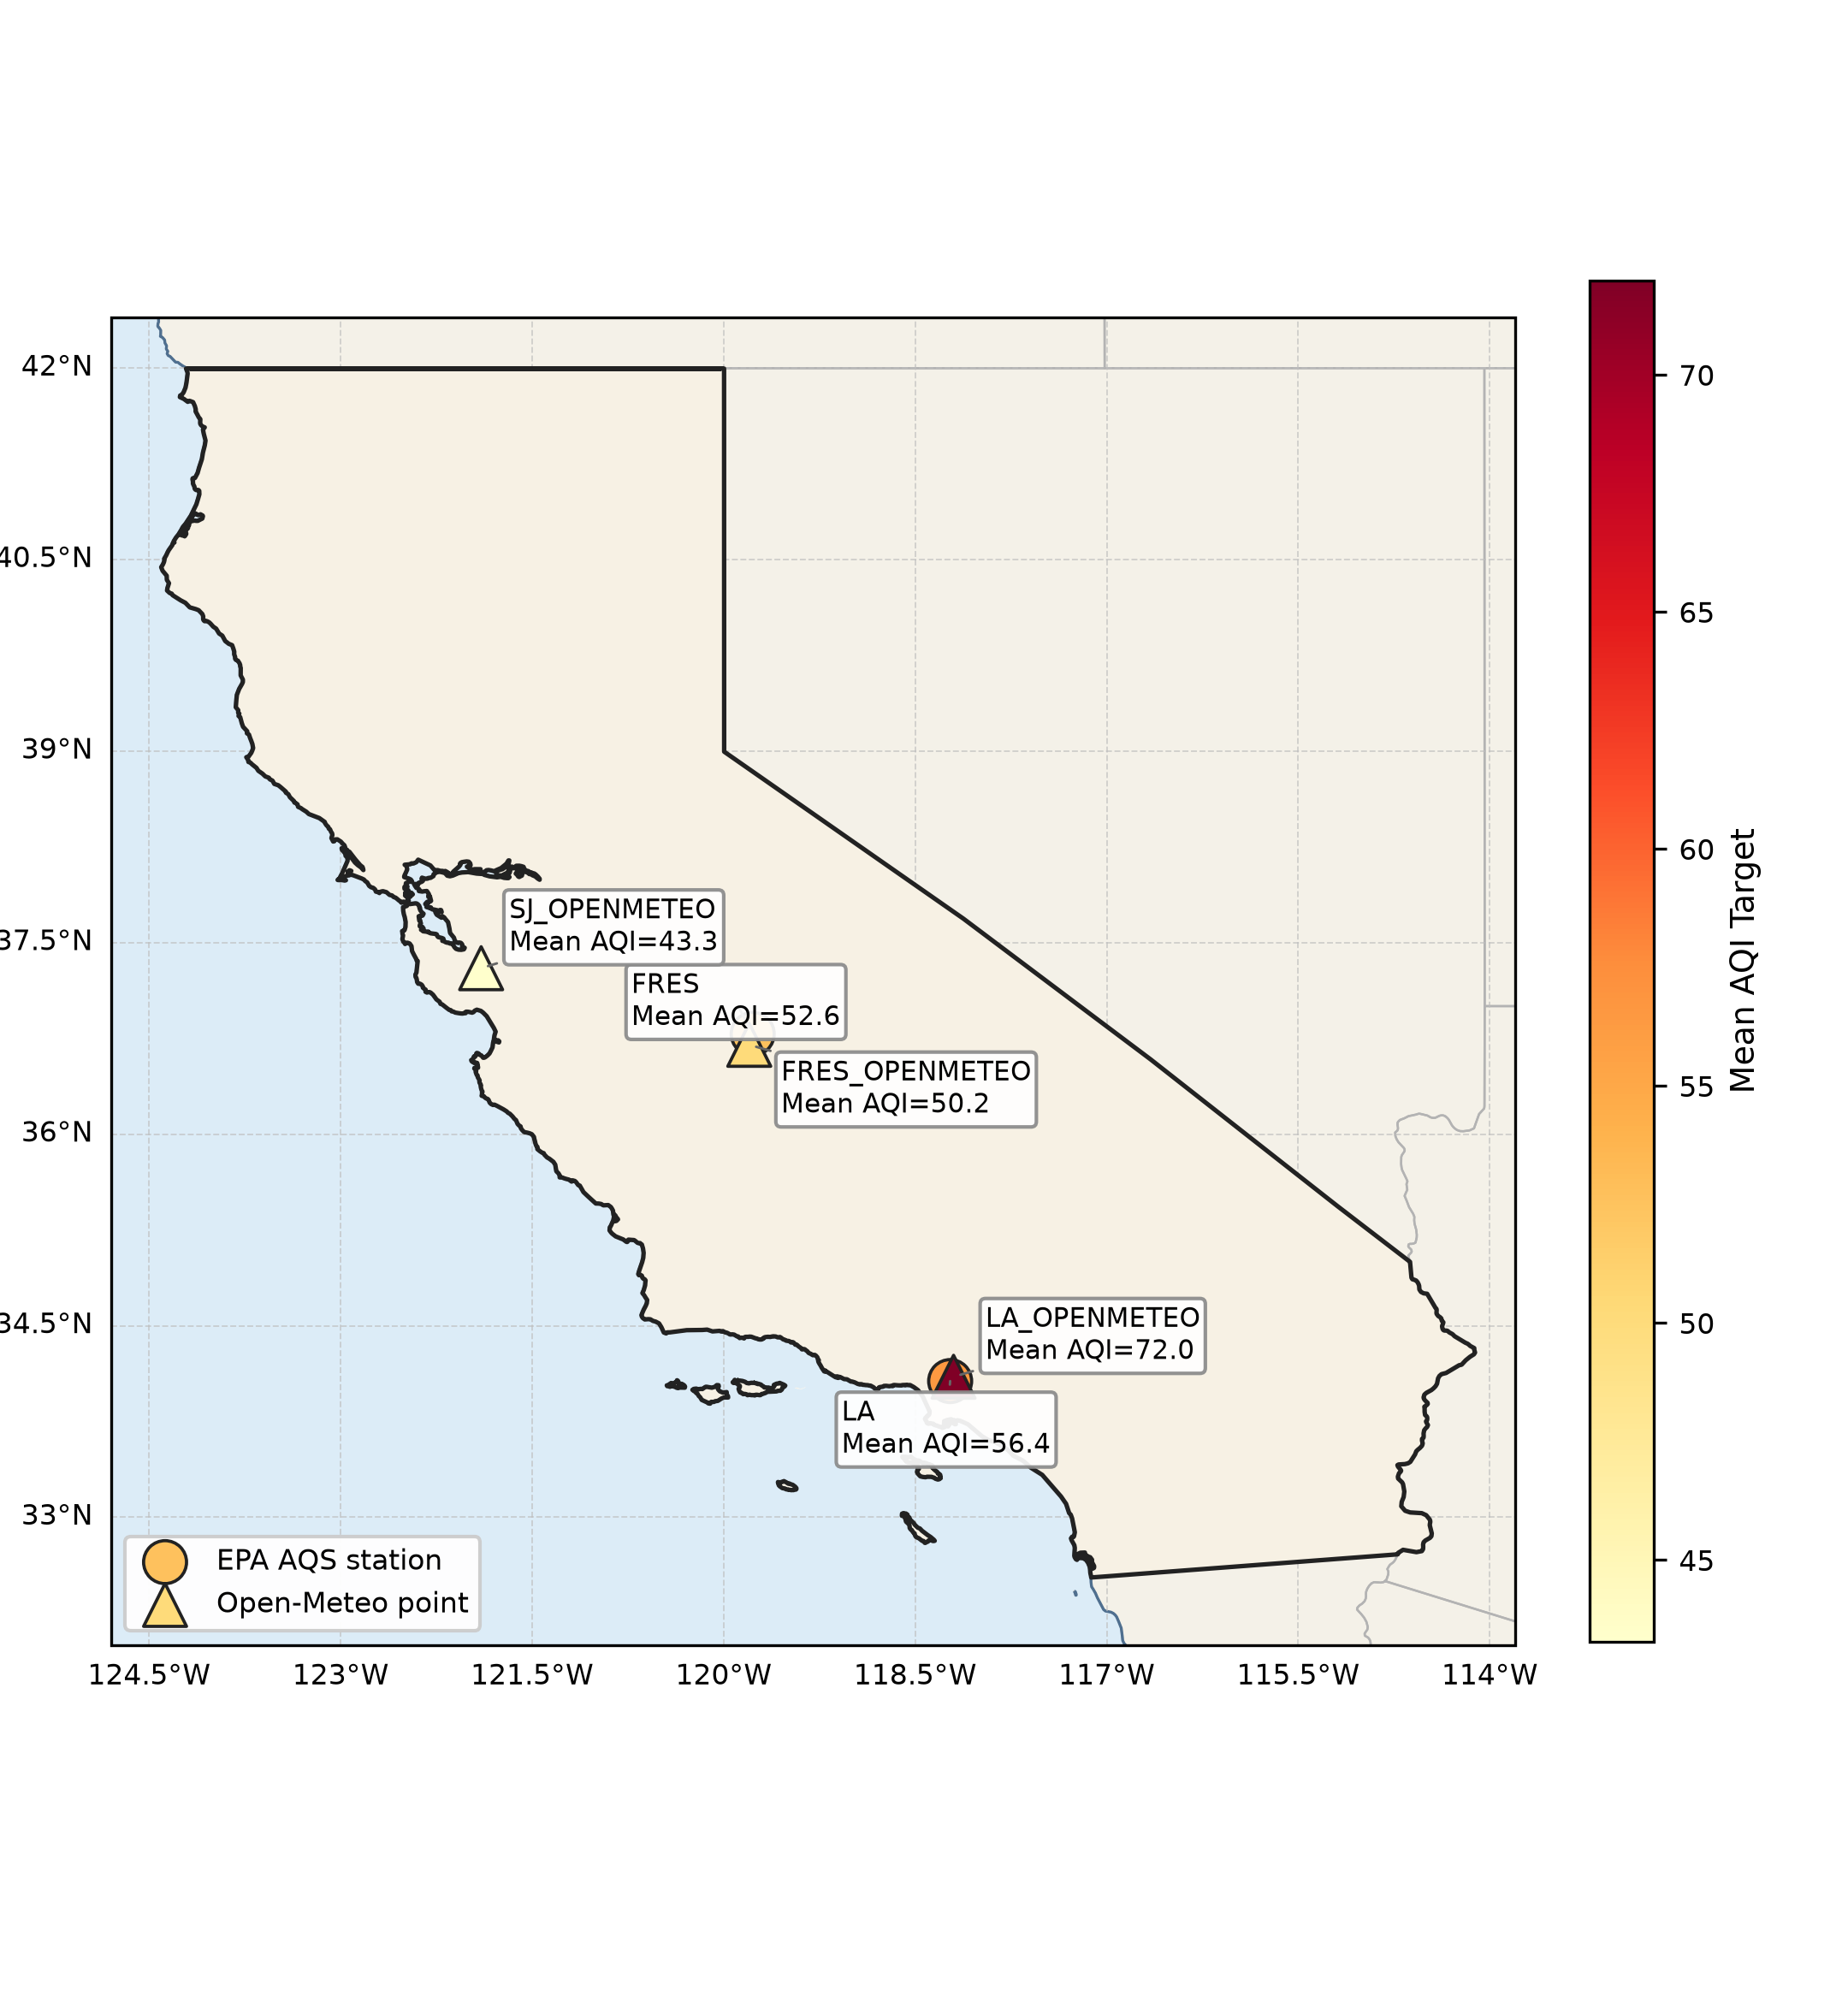
\includegraphics[width=0.65\linewidth]{figures/paper_station_map.png}
    \caption{Spatial coverage of the California AQI panel dataset.}
    \label{fig:station-map}
\end{figure}

Preprocessing yields 181,122 hourly records with 21 base attributes prior to lag expansion. The target distribution displays strong right-skewness: mean AQI is 54.79, median is 54.54, the 95th percentile reaches 97.21, and the 99th percentile hits 151.84. This heavy tail requires scenario evaluation rather than relying solely on global error averages.

\subsection{Exploratory Correlation Structure}\label{subsec:correlation}
Exploratory analysis confirms PM2.5 as the primary direct correlate of target AQI. Weather attributes provide secondary context; wind speed correlates negatively with AQI due to atmospheric dispersion. Figure~\ref{fig:correlation-heatmap} displays these relationships.

\begin{figure}[htbp]
    \centering
    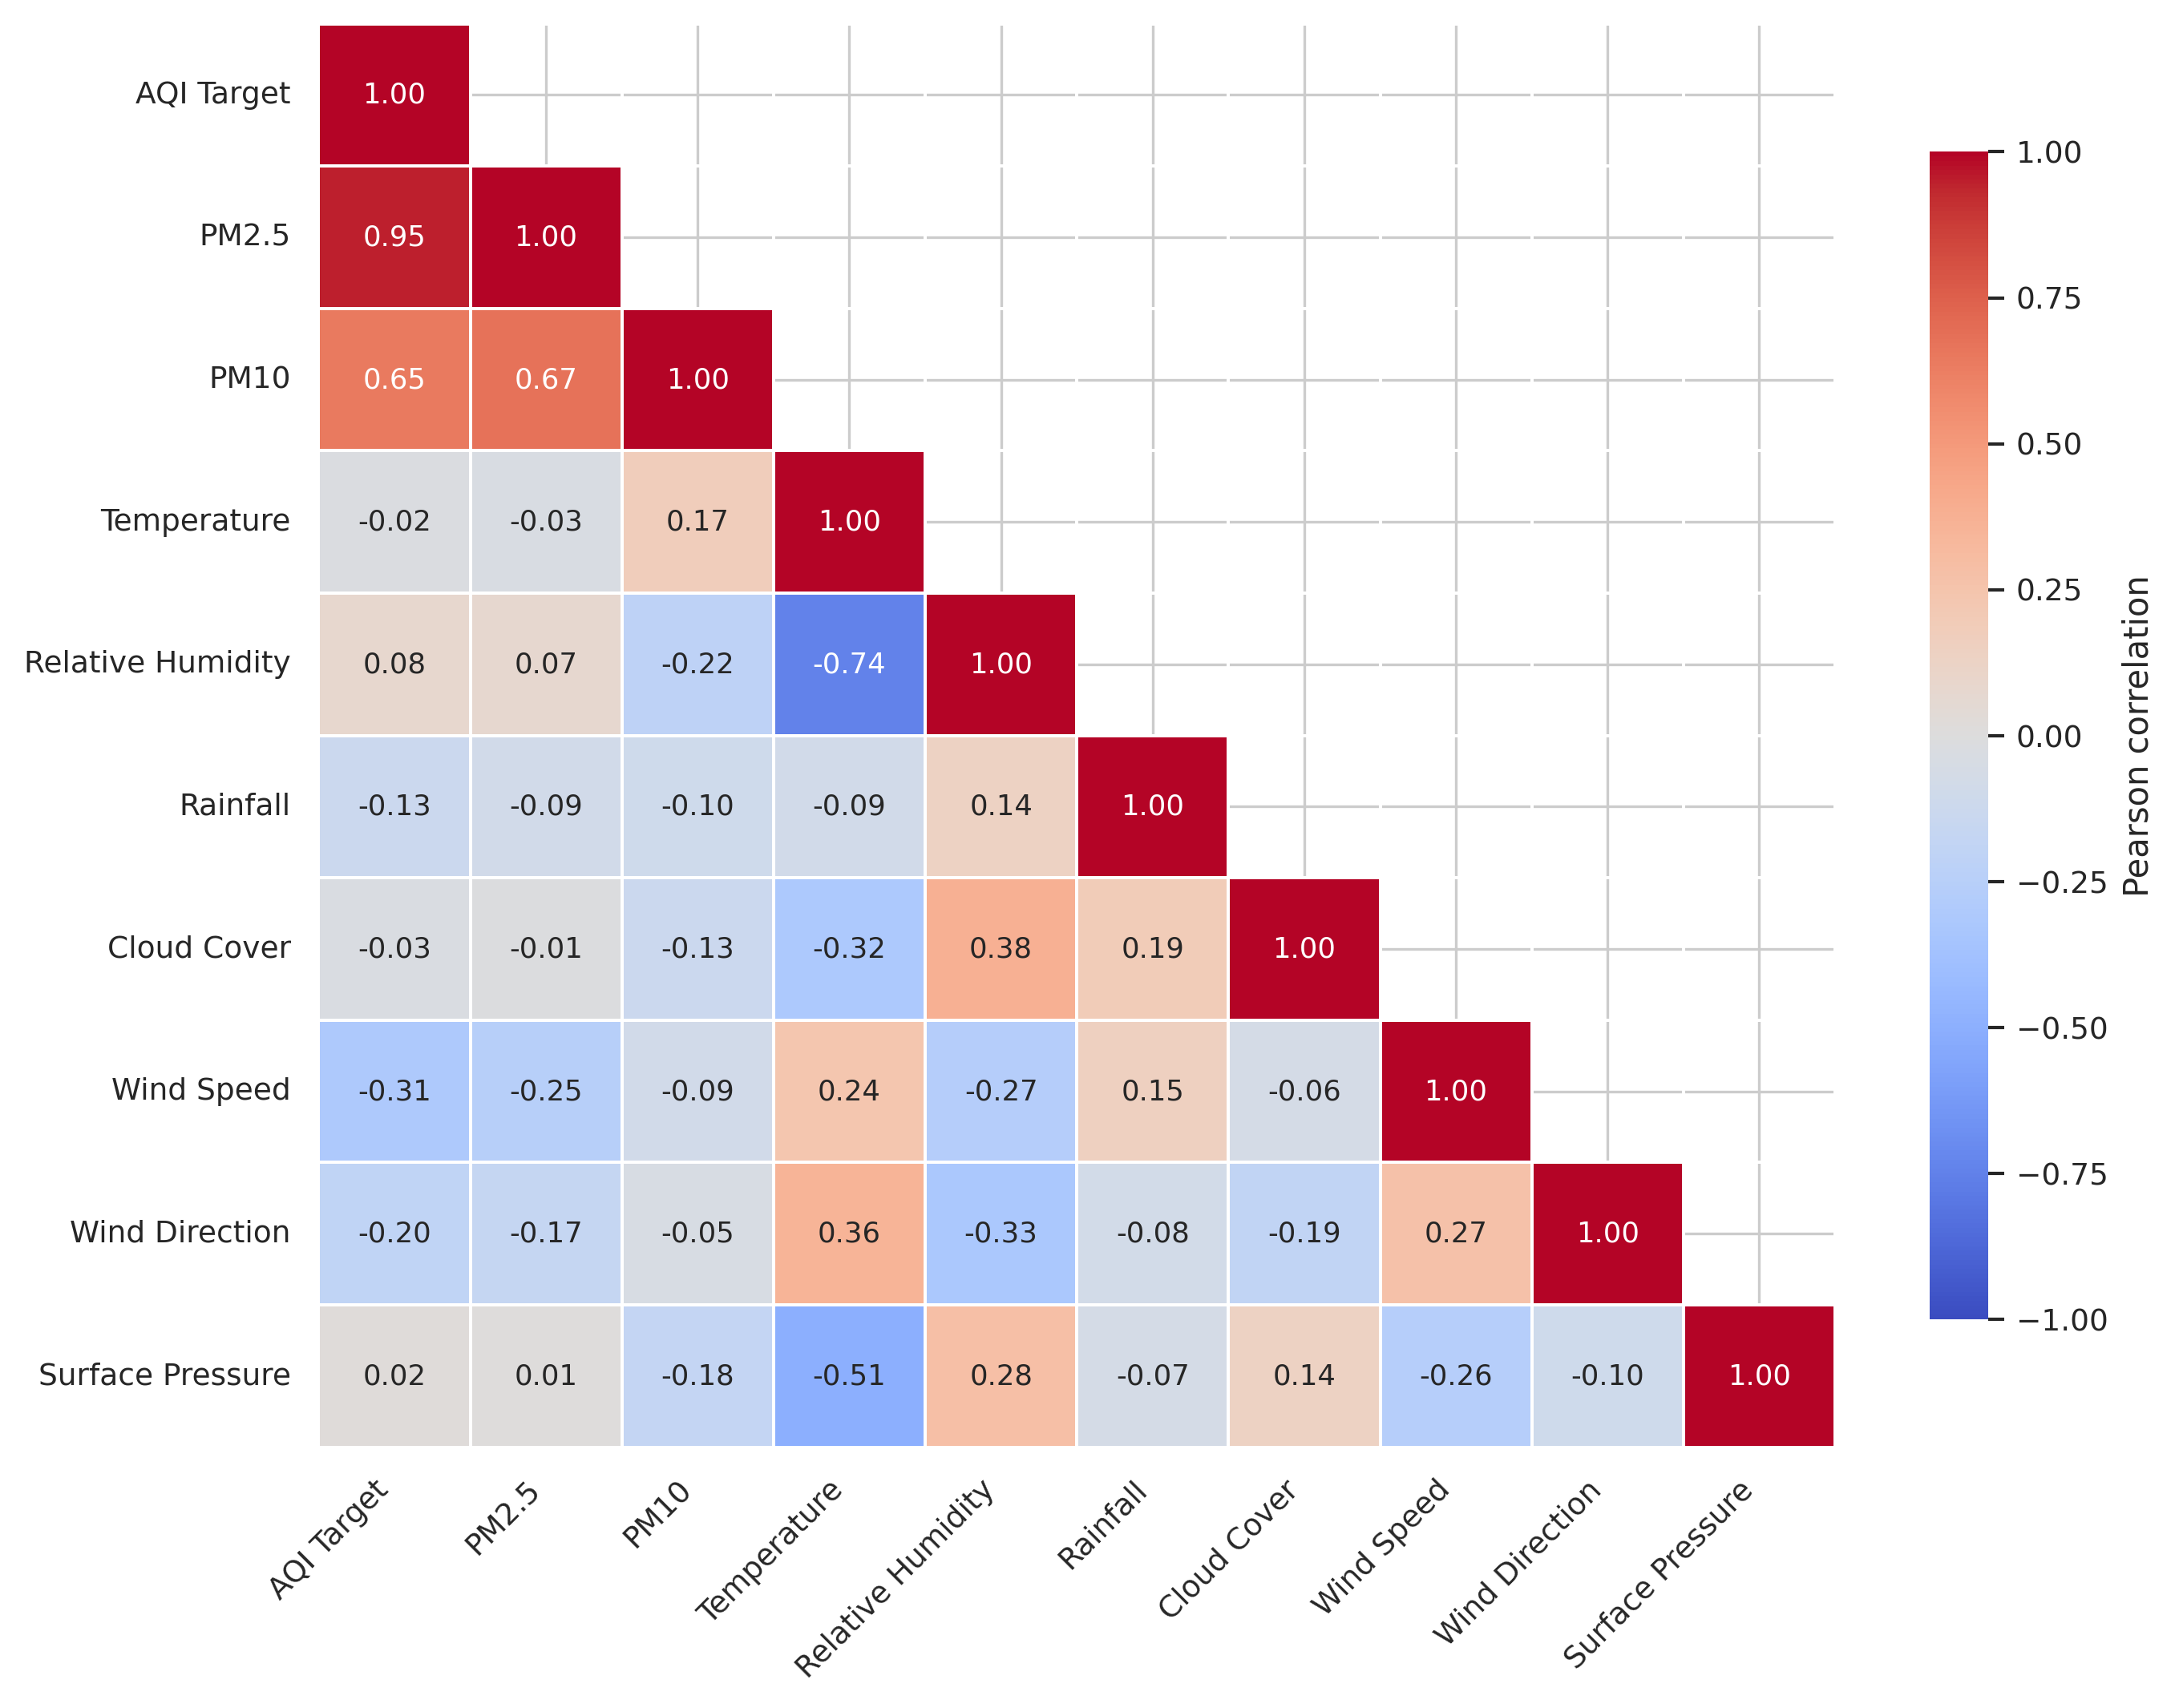
\includegraphics[width=0.78\linewidth]{figures/paper_correlation_heatmap_en.png}
    \caption{Pearson correlation heatmap for selected AQI, pollutant, and meteorological variables in the model-ready California panel.}
    \label{fig:correlation-heatmap}
\end{figure}

\section{Feature Engineering}\label{sec:feature-engineering}
\subsection{Engineered Dryness Feature: VPD}\label{subsec:vpd}
We compute Vapor Pressure Deficit (VPD) to quantify atmospheric moisture demand by comparing saturation and actual vapor pressure \cite{allen1998crop}. VPD indicates atmospheric dryness and plant water stress \cite{grossiord2020plant}. We evaluate VPD as a physical context variable rather than assuming prior accuracy gains.

Given temperature $T$ ($^\circ\text{C}$) and relative humidity $\mathrm{RH}$ (\%), saturation vapor pressure is
\begin{equation}
    e_s(T)=0.6108 \exp\left(\frac{17.27T}{T+237.3}\right).
    \label{eq:saturation-vapor-pressure}
\end{equation}
Actual vapor pressure is
\begin{equation}
    e_a(T,\mathrm{RH})=\frac{\mathrm{RH}}{100}e_s(T).
    \label{eq:actual-vapor-pressure}
\end{equation}
The engineered VPD feature is
\begin{equation}
    \mathrm{VPD}=\max\left(e_s(T)-e_a(T,\mathrm{RH}),0\right).
    \label{eq:vpd}
\end{equation}

Our exploratory code recomputes VPD from meteorological variables and generates a monthly diagnostic plot. This diagnostic verifies that the engineered dryness signal follows plausible seasonal structure before inclusion in the feature set.

\begin{figure}[htbp]
    \centering
    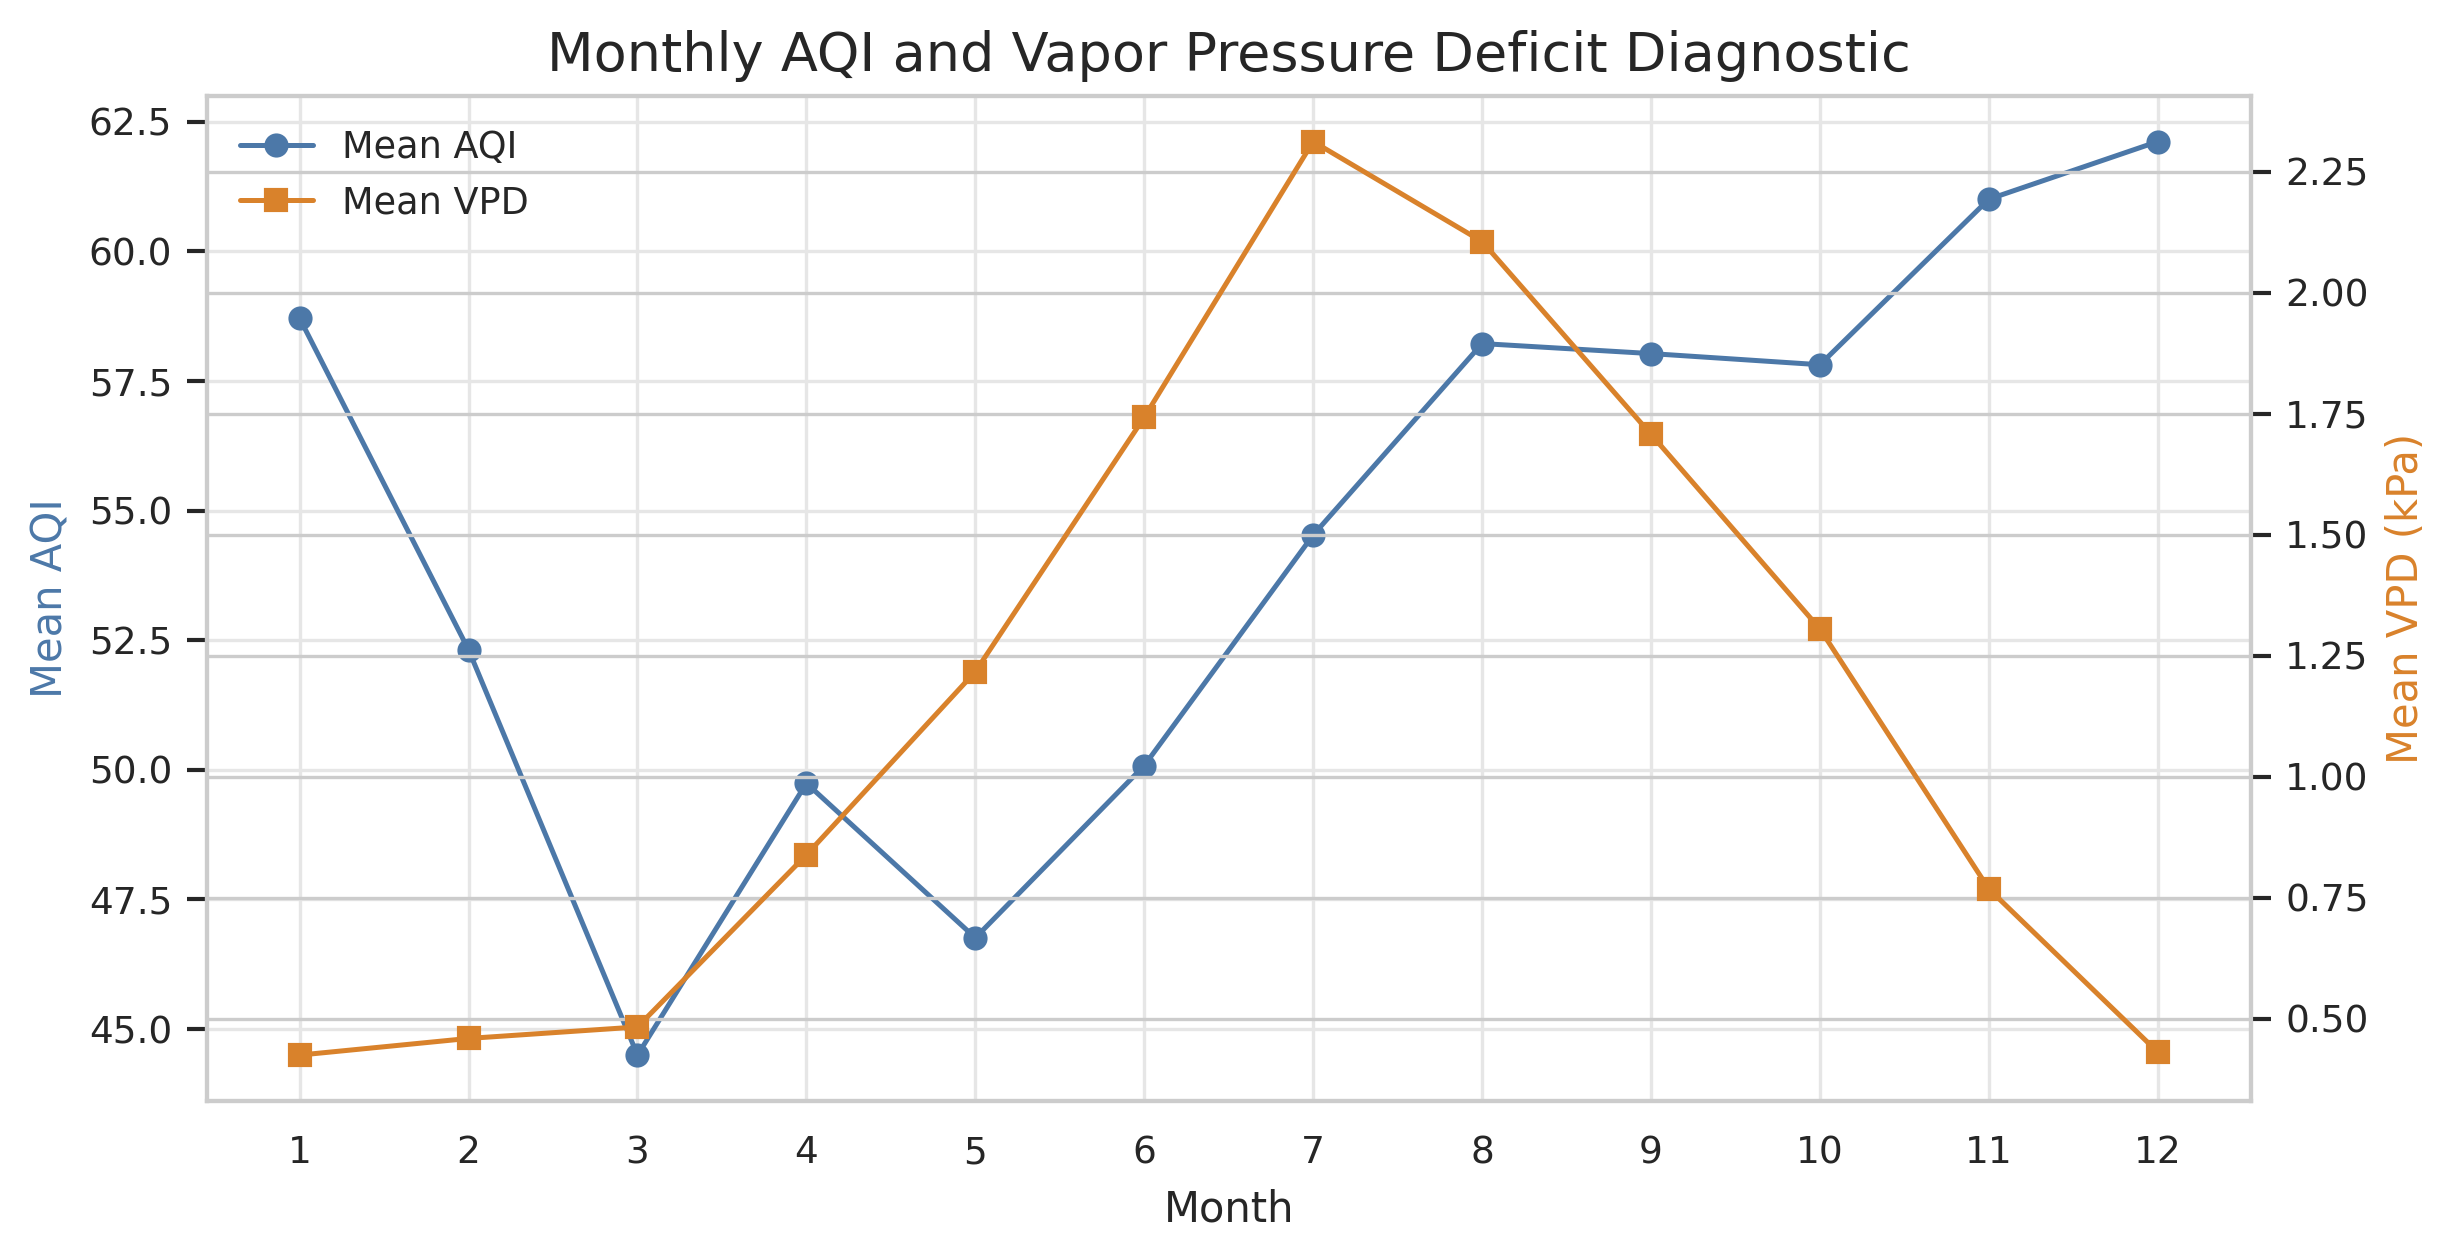
\includegraphics[width=0.82\linewidth]{figures/07_vpd_monthly_diagnostic.png}
    \caption{Monthly diagnostic of recomputed VPD, inspecting seasonal dryness structure in the AQI panel.}
    \label{fig:vpd-diagnostic}
\end{figure}

\subsection{Temporal and Spatial Lag Features}\label{subsec:lag-features}
Temporal lag features encode recent and day-prior AQI states. For station $s$ at target time $t$, a local lag feature is
\begin{equation}
    \mathrm{Lag}_{s,k}(t)=y_{s,t-k},
    \label{eq:local-lag}
\end{equation}
where $k$ is the lag horizon in hours. Spatial lag features summarize delayed AQI information from other stations:
\begin{equation}
    \mathrm{SpatialLag}_{s,k}(t)=
    \frac{1}{|\mathcal{N}(s)|}\sum_{j \in \mathcal{N}(s)} y_{j,t-k}.
    \label{eq:spatial-lag}
\end{equation}
These features provide transport-related context, and their predictive value is tested empirically in our ablation study.

Additional features include cyclic hour/month encodings, wind-vector decomposition, dry-heat interaction terms, dry-wind interaction terms, temperature-humidity ratios, and wind-speed-pressure ratios. Categorical station identifiers are retained for model families supporting categorical or one-hot encoded inputs.

\section{Methodology}\label{sec:methodology}
\subsection{Pipeline Overview}\label{subsec:pipeline}
Our workflow converts monitoring logs and weather inputs into a benchmark free of temporal leakage. Key stages include data harmonization, feature generation, chronological partitioning, model training, leaderboard scoring, scenario analysis, and ablation testing.

\begin{figure}[htbp]
    \centering
    
\includegraphics[width=0.78\linewidth]{figures/paper_workflow_pipeline_architecture.jpg}
    \caption{AQI forecasting pipeline architecture.}
    \label{fig:pipeline-architecture}
\end{figure}

\subsection{Forecasting Tasks}\label{subsec:forecasting-tasks}
For station $s$ and target time $t$, the forecasting task is formulated as
\begin{equation}
    \hat{y}_{s,t+h}=f(\mathbf{x}_{s,t}),
    \label{eq:forecasting-task}
\end{equation}
where $\hat{y}_{s,t+h}$ is predicted AQI at horizon $h$, and $\mathbf{x}_{s,t}$ contains weather features, calendar encodings, station IDs, VPD, lagged AQI, and allowed spatial context.

We evaluate two configurations:
\begin{enumerate}
    \item \textbf{Short-term nowcasting}: Uses recent local lags (1--3 hours), leveraging strong temporal autocorrelation.
    \item \textbf{24-hour forecasting}: Excludes local AQI from $t-1$ to $t-23$, forcing models to rely on weather, calendar cycles, VPD, spatial lags, and day-prior AQI.
\end{enumerate}

\subsection{Data Splitting Strategy}\label{subsec:data-split}
We enforce a chronological split to prevent temporal leakage. Random partitioning leaks lagged states and weather patterns across sets, artificially inflating performance. Table~\ref{tab:data-split} outlines the split structure.

\begin{table}[htbp]
\caption{Chronological data split used for model selection and evaluation.}\label{tab:data-split}
\begin{tabular*}{\textwidth}{@{\extracolsep\fill}lll}
\toprule
Partition & Years & Role and rationale \\
\midrule
Training & 2018, 2019, 2021--2024 & Model parameter fitting. \\
Validation & 2020 & Model selection under wildfire extremes. \\
Test & 2025 & Final independent performance reporting. \\
\botrule
\end{tabular*}
\end{table}

Isolating 2020 creates a high-smoke validation environment (August Complex fires). Unprecedented rainfall in 2022--2023 produced unusually clean air; training without extreme validation risks underestimating severe events. The 2025 test set (including the Palisades Fire) acts as the final holdout.

\subsection{Chronological Boundary Leakage Guard}\label{subsec:leakage-guard}
To prevent lag features from crossing split boundaries, we enforce a temporal buffer $G_h$:
\begin{equation}
    \Delta t_{\mathrm{boundary}} \geq G_h,
    \qquad
    G_h =
    \begin{cases}
    4 \text{ hours}, & \text{short-term nowcasting},\\
    215 \text{ hours}, & \text{long-term 24-hour forecasting}.
    \end{cases}
    \label{eq:boundary-guard}
\end{equation}
Audit checks verify that target proxies and future features are excluded.

\subsection{Models and Metrics}\label{subsec:models-metrics}
We benchmark five regressors: Linear Ridge, Random Forest, LightGBM, CatBoost, and XGBoost. CatBoost processes categorical station IDs natively, while other models use train-set scaling and encoding.

Two operational baselines benchmark performance:
\begin{itemize}
    \item \textbf{Persistence}: Projects the last available observation ($t-1$ for short-term, $t-24$ for long-term).
    \item \textbf{Climatology}: Predicts historical mean AQI per hour-of-day and month from the training set.
\end{itemize}

Evaluation metrics include Mean Absolute Error (MAE), Root Mean Squared Error (RMSE), and $R^2$:
\begin{equation}
    \mathrm{MAE}=\frac{1}{n}\sum_{i=1}^{n}|y_i-\hat{y}_i|,
    \label{eq:mae}
\end{equation}
\begin{equation}
    \mathrm{RMSE}=\sqrt{\frac{1}{n}\sum_{i=1}^{n}(y_i-\hat{y}_i)^2},
    \label{eq:rmse}
\end{equation}
\begin{equation}
    R^2=1-\frac{\sum_{i=1}^{n}(y_i-\hat{y}_i)^2}{\sum_{i=1}^{n}(y_i-\bar{y})^2}.
    \label{eq:r2}
\end{equation}

\subsection{System Architecture and Deployment}\label{subsec:system-architecture}
We deployed trained pipelines into a real-time early warning web application. A FastAPI backend handles model inference and computes SHAP values and feature gain scores for interpretability (Figure~\ref{fig:feature-importance}). An SQLite database caches Open-Meteo weather fields and EPA AQS data to minimize latency.

\begin{figure}[htbp]
    \centering
    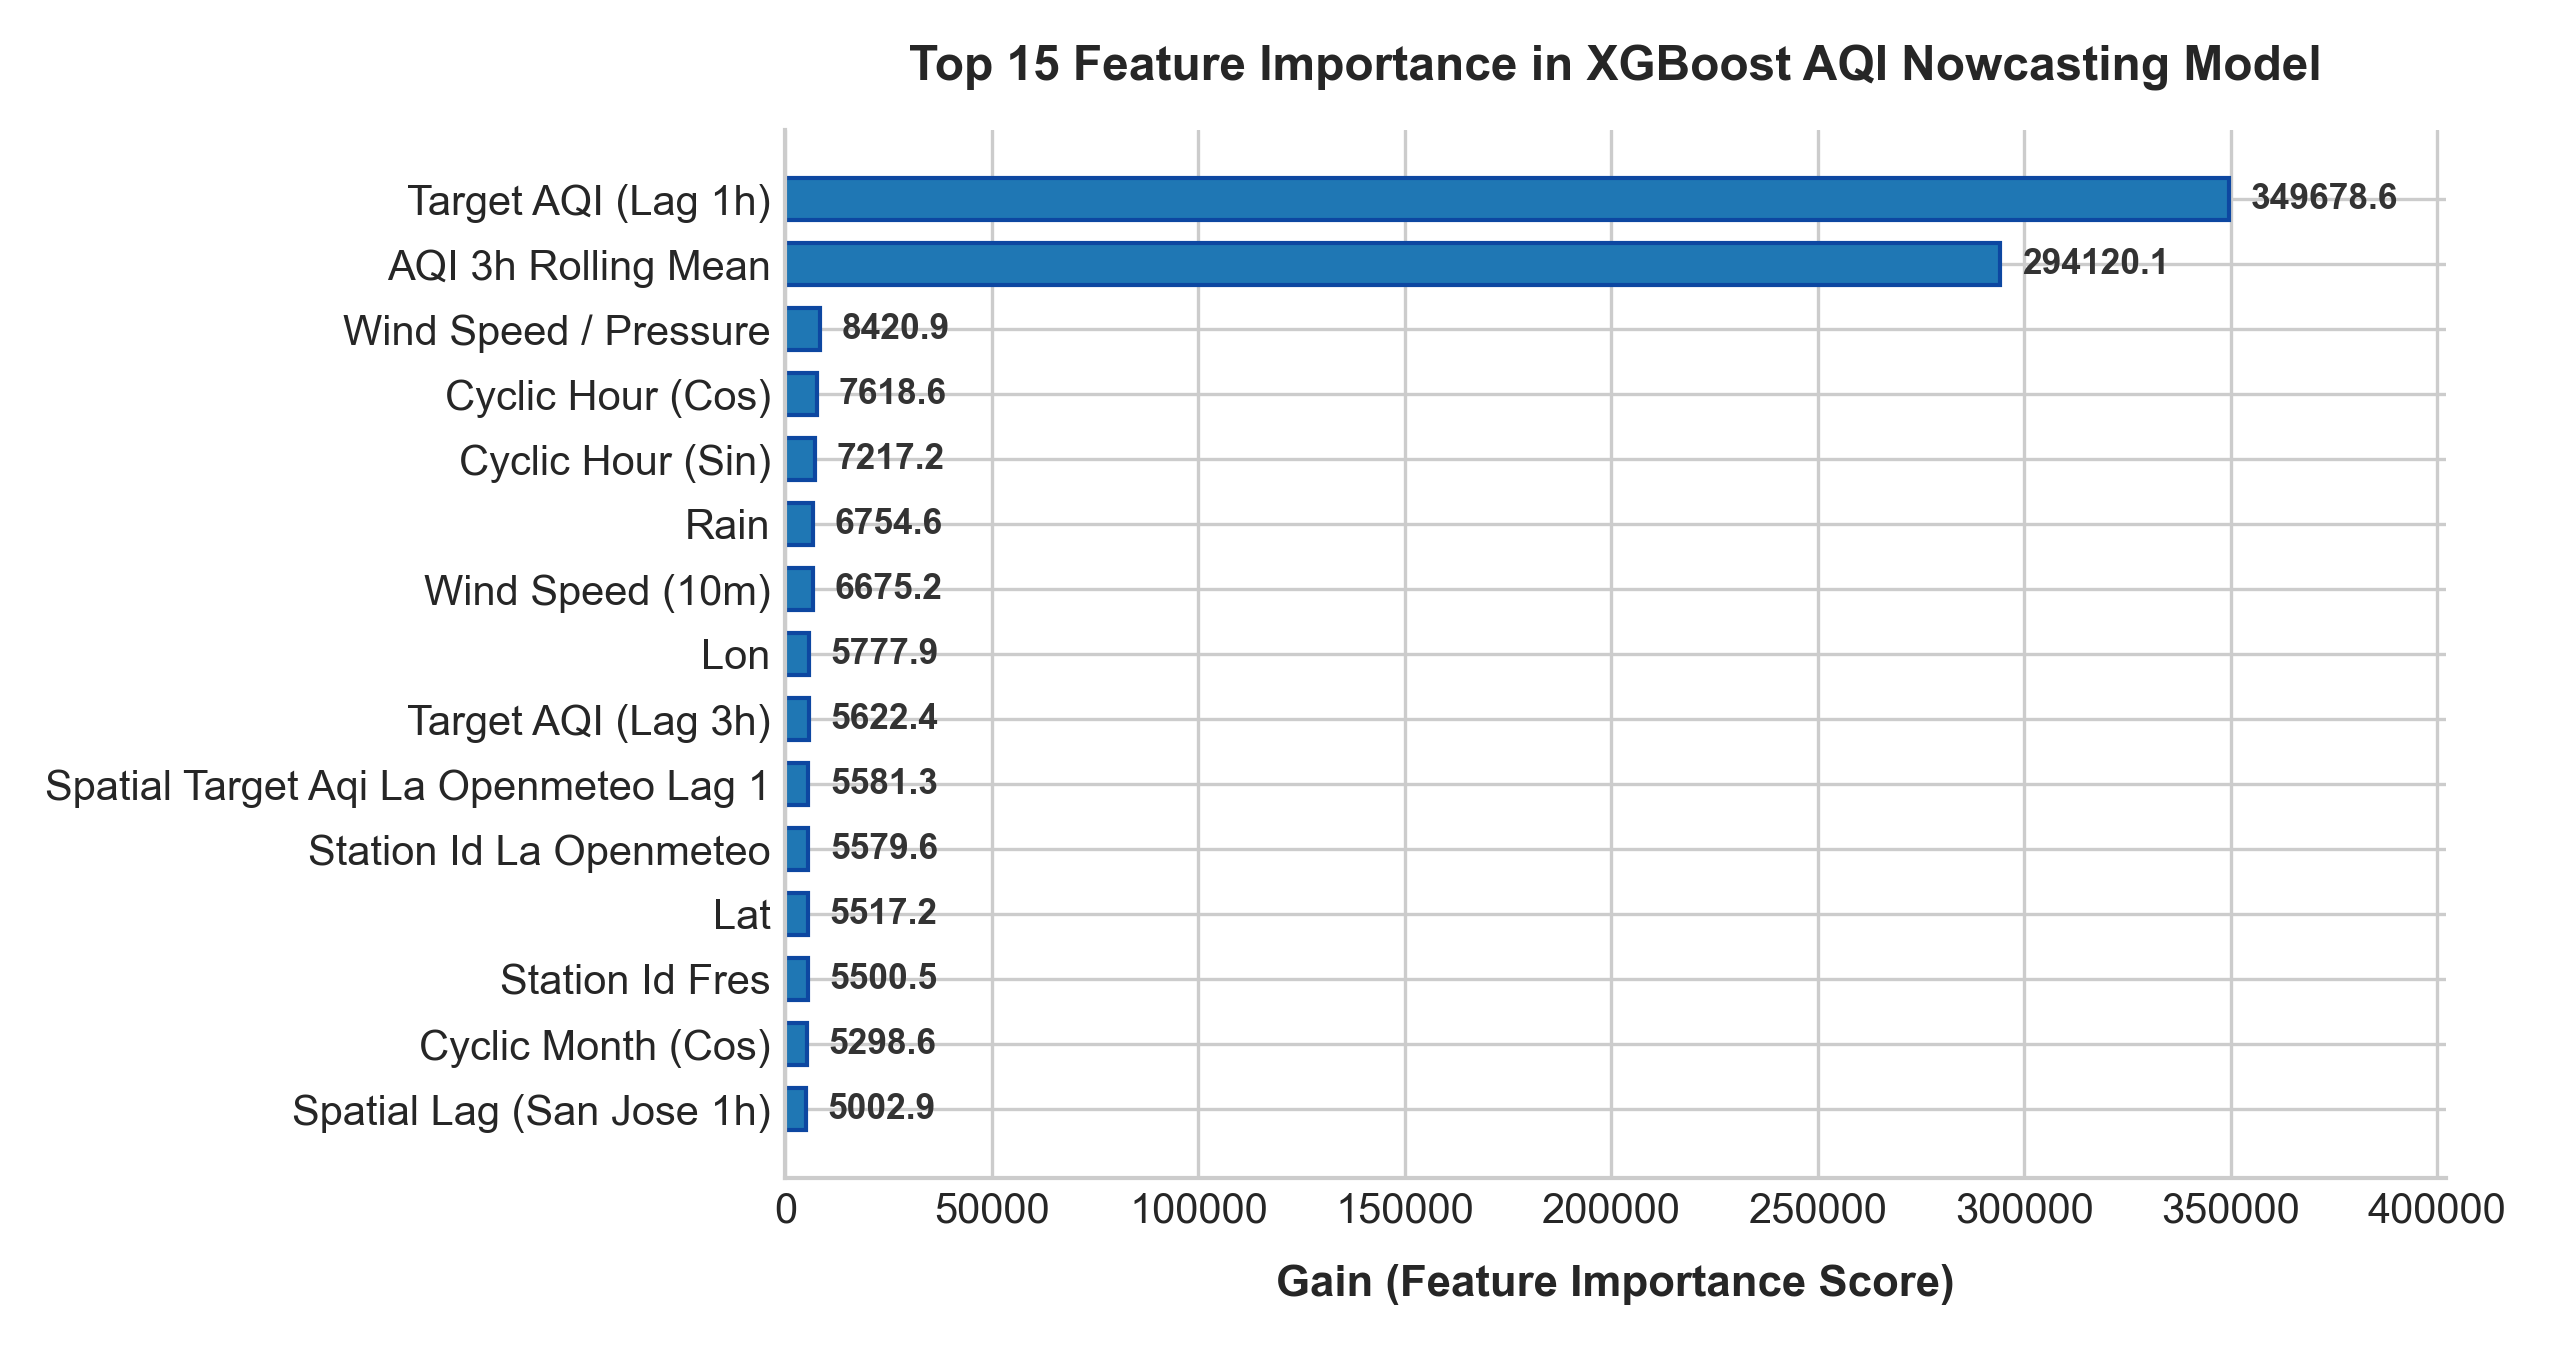
\includegraphics[width=0.80\linewidth]{figures/paper_shap_feature_importance.png}
    \caption{Top 15 feature importances (gain scores) for the primary XGBoost nowcasting model, highlighting the dominance of short-term local lags, VPD, and weather ratios.}
    \label{fig:feature-importance}
\end{figure}

The Streamlit frontend displays interactive PyDeck heatmaps of AQI across Fresno, Los Angeles, and San Jose. It provides side-by-side timeline plots of actual versus predicted AQI. KPI summary cards trigger automated "Air Stagnation Alerts" during deteriorating weather or predicted AQI spikes (Figure~\ref{fig:dashboard-ui}).

\begin{figure}[htbp]
    \centering
    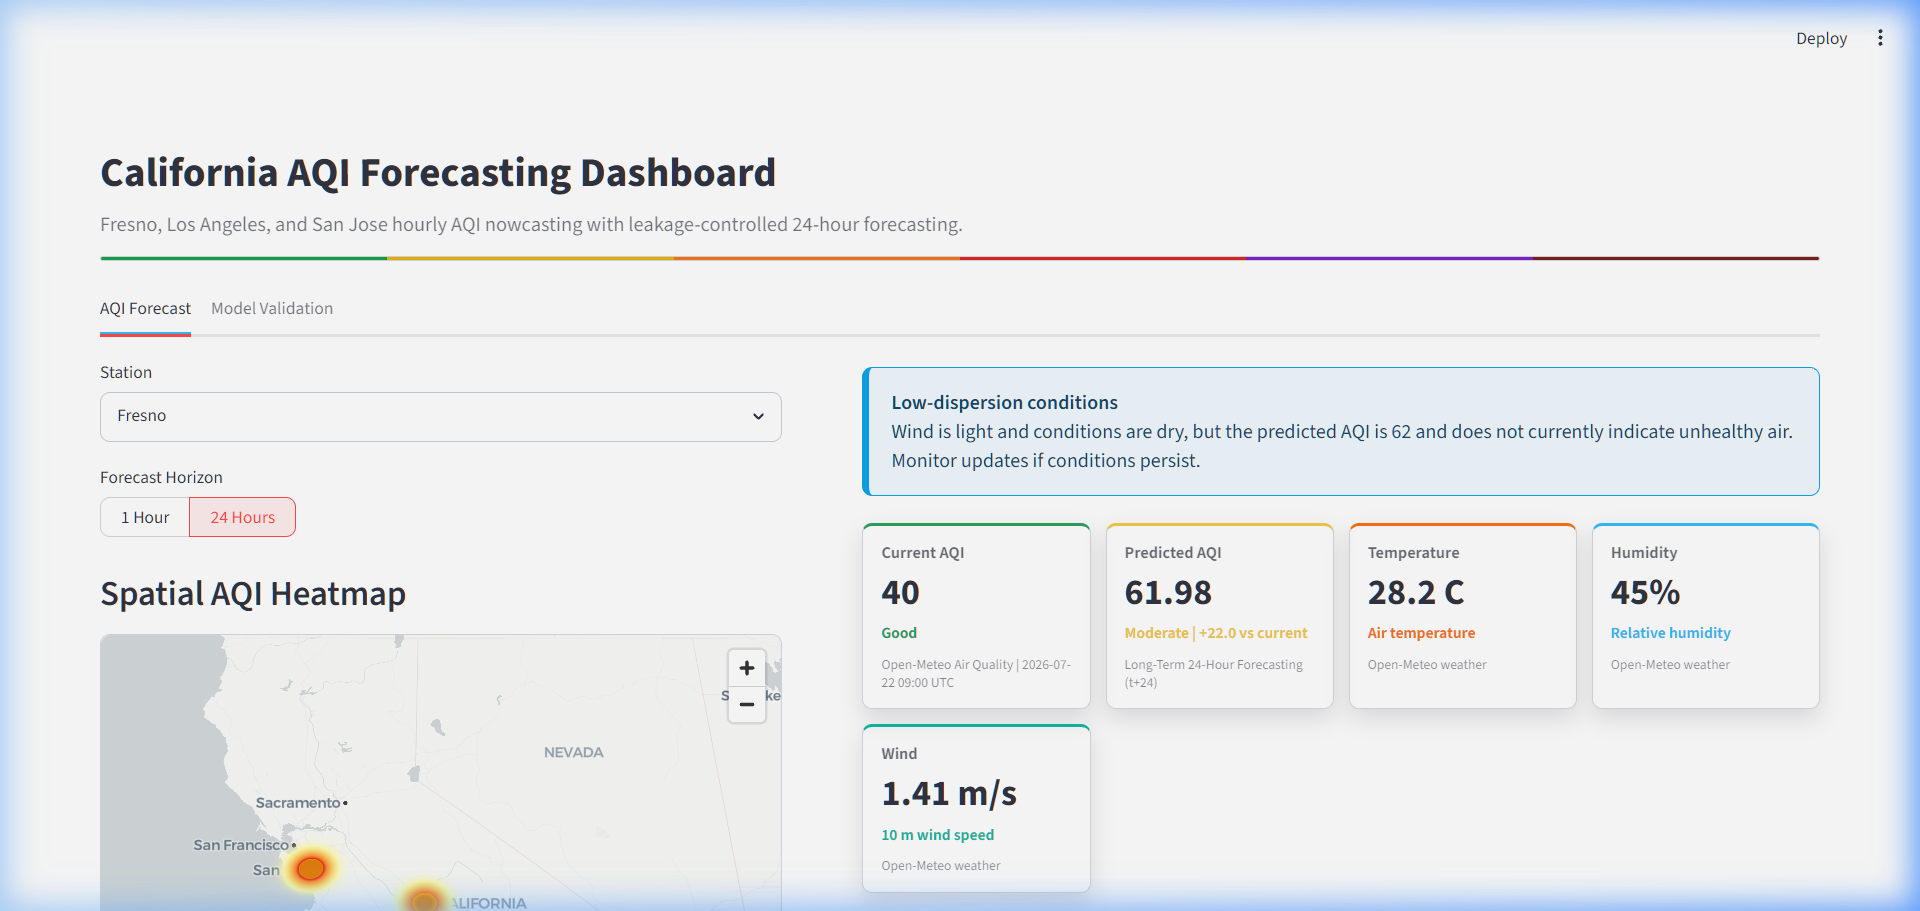
\includegraphics[width=0.85\linewidth]{figures/paper_dashboard_ui.png}
    \caption{Real-time early warning web application UI showing the PyDeck spatial AQI heatmap, atmospheric condition indicators, short-term and 24-hour prediction metrics, and automated alert panels.}
    \label{fig:dashboard-ui}
\end{figure}

\section{Results and Discussion}\label{sec:results}
\subsection{Overall Leaderboard}\label{subsec:leaderboard}
The 2025 test leaderboard highlights clear differences between horizons. Near-term nowcasting yields high $R^2$ values across all models, whereas 24-hour forecasting drops sharply in accuracy.

\subsection{Short-Term Autocorrelation Dominates Near-Term Nowcasting}\label{subsec:short-term}
Table~\ref{tab:short-results} summarizes short-term nowcasting performance. Strong autocorrelation enables all models—including naive Persistence—to achieve $R^2 > 0.85$.

\begin{table}[htbp]
\caption{Short-term autoregressive nowcasting results on the 2025 test year compared with the Reference Baseline Literature (RBL).}\label{tab:short-results}
\begin{tabular*}{\textwidth}{@{\extracolsep\fill}lrrr}
\toprule
Model & MAE & RMSE & $R^2$ \\
\midrule
XGBoost & 5.8321 & 9.4719 & 0.8711 \\
LightGBM & 6.0630 & 9.4897 & 0.8706 \\
Linear Ridge & 6.3248 & 9.6697 & 0.8657 \\
CatBoost & 6.2373 & 9.9989 & 0.8564 \\
Persistence & 6.5068 & 10.0480 & 0.8550 \\
Random Forest & 6.6052 & 10.1227 & 0.8528 \\
Vu et al.~\cite{vu2022geostationary} (RBL)* & -- & -- & 0.8500 \\
Climatology & 19.3641 & 27.0662 & $-$0.0525 \\
\botrule
\end{tabular*}
\begin{tablenotes}
\item \textit{Note}: *RBL baseline by Vu et al.\ (2022) reported 10-fold temporal cross-validation $R^2 = 0.8500$ using satellite AOD and HRRR meteorology during the 2018 Camp Fire.
\end{tablenotes}
\end{table}

XGBoost achieves the top $R^2$ (0.8711) and lowest MAE. Persistence outperforms Random Forest and matches CatBoost, reflecting strong short-term temporal autocorrelation (0.927 correlation between target and 1-hour lag). Climatology fails ($R^2 = -0.0525$), missing transient spikes.

\subsection{Horizon Degradation in 24-Hour Forecasting}\label{subsec:long-term}
Table~\ref{tab:long-results} presents 24-hour horizon performance. Excluding local lags from $t-1$ to $t-23$ forces models to rely on weather, calendar patterns, VPD, and spatial lags.

\begin{table}[htbp]
\caption{Long-term 24-hour forecasting results on the 2025 test year.}\label{tab:long-results}
\begin{tabular*}{\textwidth}{@{\extracolsep\fill}lrrr}
\toprule
Model & MAE & RMSE & $R^2$ \\
\midrule
XGBoost & 13.6366 & 19.3007 & 0.4648 \\
LightGBM & 13.5828 & 19.3349 & 0.4629 \\
Linear Ridge & 13.5179 & 19.3861 & 0.4601 \\
Random Forest & 13.9665 & 19.7806 & 0.4379 \\
CatBoost & 13.6376 & 20.2404 & 0.4114 \\
Persistence & 16.3495 & 23.1401 & 0.2307 \\
Climatology & 20.1250 & 28.0628 & $-$0.1314 \\
\botrule
\end{tabular*}
\end{table}

XGBoost leads ($R^2 = 0.4648$), followed closely by LightGBM and Linear Ridge. Persistence drops to $R^2 = 0.2307$, reflecting substantial 24-hour AQI shifts.

\subsection{Upper-Tail Extreme Spikes Reveal Model Vulnerability}\label{subsec:extreme-event}
Global metrics mask operational vulnerabilities. Figure~\ref{fig:aqi-category-timeline} illustrates AQI category shifts, highlighting high-pollution episodes.

\begin{figure}[htbp]
    \centering
    
\includegraphics[width=0.82\linewidth]{figures/eda_aqi_category_timeline.png}
    \caption{Daily AQI observations colored by U.S. AQI health category.}
    \label{fig:aqi-category-timeline}
\end{figure}

Table~\ref{tab:scenario-context-results} evaluates top models across specific scenario slices.

\begin{table}[htbp]
\caption{Best-per-scenario results for extreme-event and climate-context evaluation on the 2025 test year.}\label{tab:scenario-context-results}
\footnotesize
\setlength{\tabcolsep}{2pt}
\begin{tabular*}{\textwidth}{@{\extracolsep\fill}lllrrrr}
\toprule
Configuration & Scenario slice & Best model & $N$ & MAE & RMSE & $R^2$ \\
\midrule
Short-term & Full 2025 test year & XGBoost & 26293 & 5.8321 & 9.4719 & 0.8711 \\
Short-term & Non-event baseline (AQI $\leq 100$) & XGBoost & 24806 & 5.1739 & 7.4436 & 0.8521 \\
Short-term & January 2025 Winter Extreme Window & Linear Ridge & 1795 & 9.2156 & 14.2454 & 0.8473 \\
Short-term & Extreme AQI in 2025 (top 5\%) & Persistence & 1321 & 17.0277 & 23.0052 & 0.3004 \\
Short-term & July--September 2025 wildfire season & Persistence & 6624 & 5.9556 & 10.0932 & 0.8595 \\
Long-term & Full 2025 test year & XGBoost & 26224 & 13.6366 & 19.3007 & 0.4648 \\
Long-term & Non-event baseline (AQI $\leq 100$) & CatBoost & 24756 & 11.2602 & 14.5048 & 0.4392 \\
Long-term & January 2025 Winter Extreme Window & LightGBM & 1726 & 19.4994 & 32.7758 & 0.2103 \\
Long-term & Extreme AQI in 2025 (top 5\%) & Persistence & 1315 & 39.3547 & 51.7407 & $-$2.3742 \\
Long-term & July--September 2025 wildfire season & Random Forest & 6624 & 13.3133 & 18.9501 & 0.5047 \\
\botrule
\end{tabular*}
\end{table}

Three insights emerge. First, Persistence outperforms machine learning models on short-term top-5\% AQI and Wildfire slices. Second, short-term top-5\% $R^2$ drops to 0.3004. Third, 24-hour top-tail forecasts yield negative $R^2$ across all models (Persistence: $-2.3742$). Without smoke plume or fire perimeter inputs, weather and lag features cannot anticipate abrupt upper-tail spikes.

\subsection{Prediction Diagnostics}\label{subsec:diagnostics}
Figure~\ref{fig:predicted-vs-actual-comparison} compares predicted versus actual AQI scatter plots for both XGBoost and LightGBM. While central values match closely along the 1:1 identity line, high-AQI peaks display dispersion across both gradient boosting architectures.

\begin{figure}[htbp]
    \centering
    \begin{minipage}{0.48\linewidth}
        \centering
        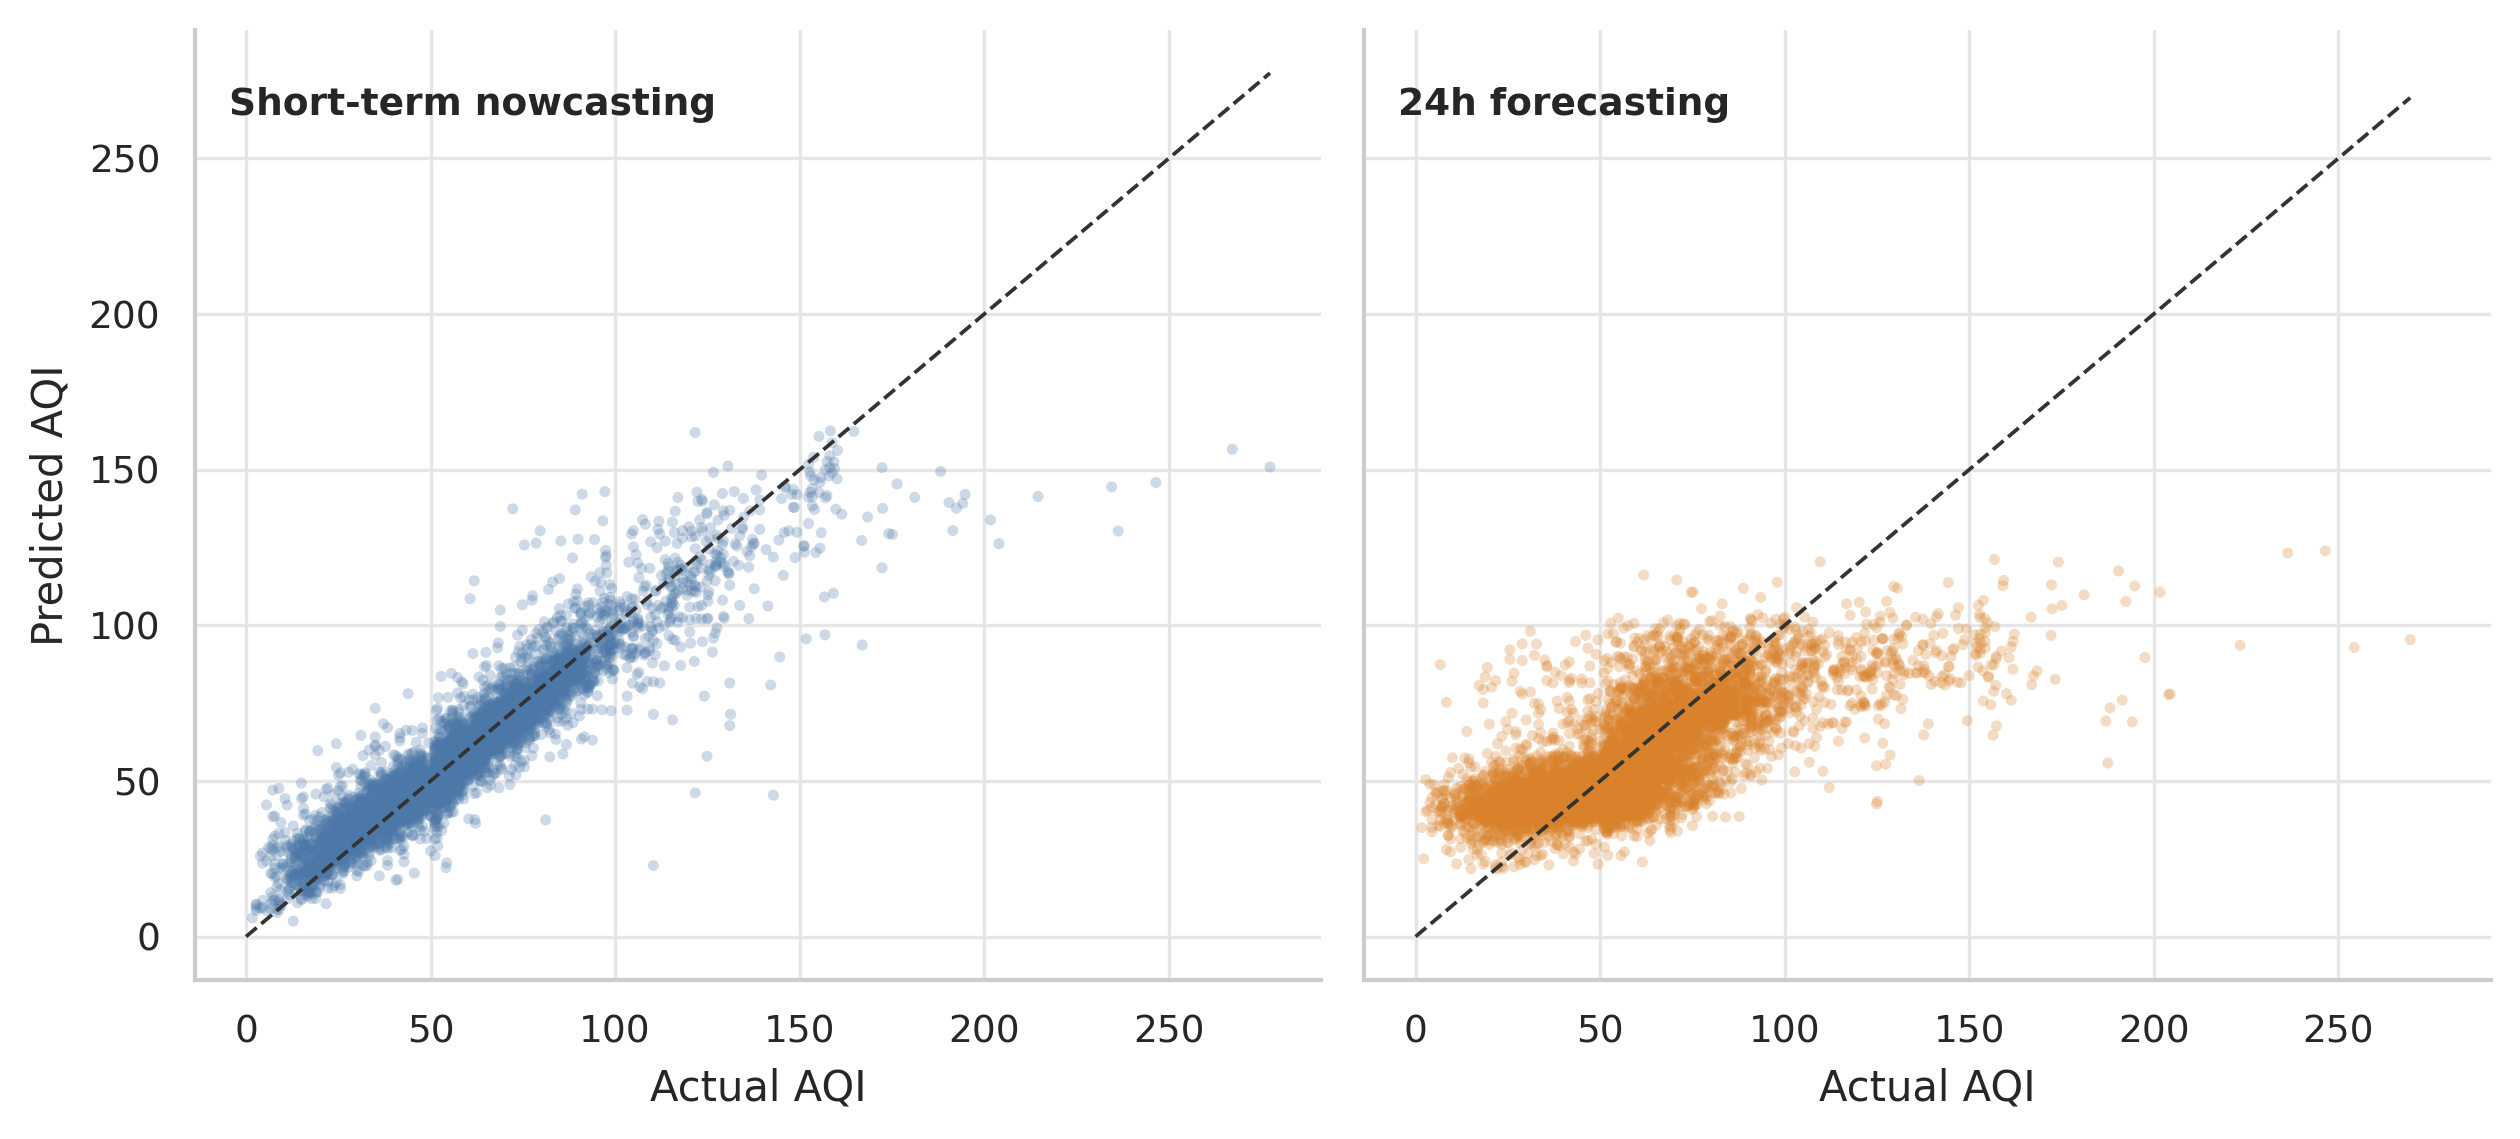
\includegraphics[width=\linewidth]{figures/paper_xgboost_predicted_vs_actual.png}
        \centerline{\small (a) XGBoost ($R^2 = 0.8711$)}
    \end{minipage}\hfill
    \begin{minipage}{0.48\linewidth}
        \centering
        
\includegraphics[width=\linewidth]{figures/paper_lightgbm_predicted_vs_actual.png}
        \centerline{\small (b) LightGBM ($R^2 = 0.8706$)}
    \end{minipage}
    \caption{Predicted versus actual AQI scatter diagnostics on the independent 2025 test year for top-performing gradient boosted decision tree regressors.}
    \label{fig:predicted-vs-actual-comparison}
\end{figure}

\subsection{Comparison with Reference Baseline Literature (RBL)}\label{subsec:rbl-comparison}
We contextualize our empirical results against the reference baseline literature (RBL) by Vu et al.~\cite{vu2022geostationary}, who modeled PM2.5 levels during the 2018 California Camp Fire using a satellite-augmented Random Forest framework.

Vu et al.\ achieved a temporal cross-validation $R^2$ of 0.8500 and an out-of-bag $R^2$ of 0.9200 by integrating high-resolution GOES-16 satellite Aerosol Optical Depth (AOD), HRRR meteorology, and SMOTE oversampling. In our benchmark, our top short-term nowcasting model (XGBoost) achieves a comparable test $R^2$ of 0.8711 (and Random Forest achieves $R^2 = 0.8528$), validating that tabular meteorological attributes paired with autoregressive AQI lags match near-term estimation performance.

\begin{table}[htbp]
\caption{Comparative overview of our benchmark models against the Reference Baseline Literature (RBL) by Vu et al.~\cite{vu2022geostationary}.}\label{tab:rbl-comparison}
\footnotesize
\setlength{\tabcolsep}{2pt}
\begin{tabular*}{\textwidth}{@{\extracolsep\fill}lllll}
\toprule
Study / Model & Target / Scope & Key Feature Inputs & Validation Scheme & Test/CV $R^2$ \\
\midrule
Vu et al.~\cite{vu2022geostationary} (RBL RF) & 2018 Camp Fire & AQS + GOES-16 AOD + HRRR & Out-of-Bag (OOB) & 0.9200 \\
Vu et al.~\cite{vu2022geostationary} (RBL RF) & 2018 Camp Fire & AQS + GOES-16 AOD + HRRR & 10-Fold Temporal CV & 0.8500 \\
\midrule
Ours: XGBoost (Short-Term) & 2025 Hourly AQI & AQS + Open-Meteo + Lags & 2025 Test Set & \textbf{0.8711} \\
Ours: Random Forest (Short-Term) & 2025 Hourly AQI & AQS + Open-Meteo + Lags & 2025 Test Set & 0.8528 \\
Ours: XGBoost (24-Hour) & 2025 Hourly AQI & Open-Meteo + Prior Lags & 2025 Test Set & 0.4648 \\
Ours: Short-Term (Top 5\% Slice) & 2025 Upper Tail & AQS + Open-Meteo + Lags & Scenario Slice & 0.3004 \\
Ours: 24-Hour (Top 5\% Slice) & 2025 Upper Tail & Open-Meteo + Prior Lags & Scenario Slice & $-$2.3742 \\
\botrule
\end{tabular*}
\end{table}

Two key operational insights emerge:
\begin{enumerate}
    \item \textbf{Horizon Degradation}: While Vu et al.\ focused on short-term PM2.5 estimation during active fire windows, extending evaluation to a strict 24-hour horizon yields performance reduction ($R^2 = 0.4648$ for XGBoost).
    \item \textbf{Extreme-Event Tail Vulnerability}: Under upper-tail extreme scenarios (top 5\% AQI spikes), short-term accuracy drops to $R^2 = 0.3004$, and 24-hour predictions yield negative $R^2$. Tabular weather and lag features alone cannot anticipate sudden wildfire smoke transport without real-time satellite AOD and active fire perimeter inputs.
\end{enumerate}

\section{Ablation Study}\label{sec:ablation}
Table~\ref{tab:ablation} reports LightGBM ablation results removing VPD and spatial lags.

\begin{table}[htbp]
\caption{LightGBM ablation study for VPD and spatial lag features on the 2025 test year.}\label{tab:ablation}
\footnotesize
\setlength{\tabcolsep}{2pt}
\begin{tabular*}{\textwidth}{@{\extracolsep\fill}llrrrrrr}
\toprule
Configuration & Feature set & Features & MAE & RMSE & $R^2$ & $\Delta$MAE & $\Delta R^2$ \\
\midrule
Short-term & Full feature set & 47 & 6.0630 & 9.4897 & 0.8706 & 0.0000 & 0.0000 \\
Short-term & Without VPD & 46 & 6.0901 & 9.5485 & 0.8690 & 0.0271 & $-$0.0016 \\
Short-term & Without spatial lags & 32 & 6.1245 & 9.4834 & 0.8708 & 0.0615 & 0.0002 \\
Long-term & Full feature set & 49 & 13.5828 & 19.3349 & 0.4629 & 0.0000 & 0.0000 \\
Long-term & Without VPD & 48 & 13.6113 & 19.3162 & 0.4640 & 0.0285 & 0.0010 \\
Long-term & Without spatial lags & 34 & 13.5542 & 19.1877 & 0.4711 & $-$0.0286 & 0.0081 \\
\botrule
\end{tabular*}
\end{table}

Removing VPD alters $R^2$ by $< 0.003$ across settings. VPD acts as an interpretable dryness descriptor rather than a standalone accuracy driver. Spatial lags show mixed impact: removing them slightly improves short-term $R^2$ while marginally raising long-term MAE.

\section{Extreme-Event Analysis}\label{sec:extreme-analysis}
We define extreme AQI using the 99th percentile threshold:
\begin{equation}
    y_t > P_{99} = 151.84.
    \label{eq:extreme-threshold}
\end{equation}
This isolates 1,802 extreme hourly records (0.99\% of data). Year 2020 accounts for the largest share, with August--October containing 42.8\% of extreme hours.

\begin{figure}[htbp]
    \centering
    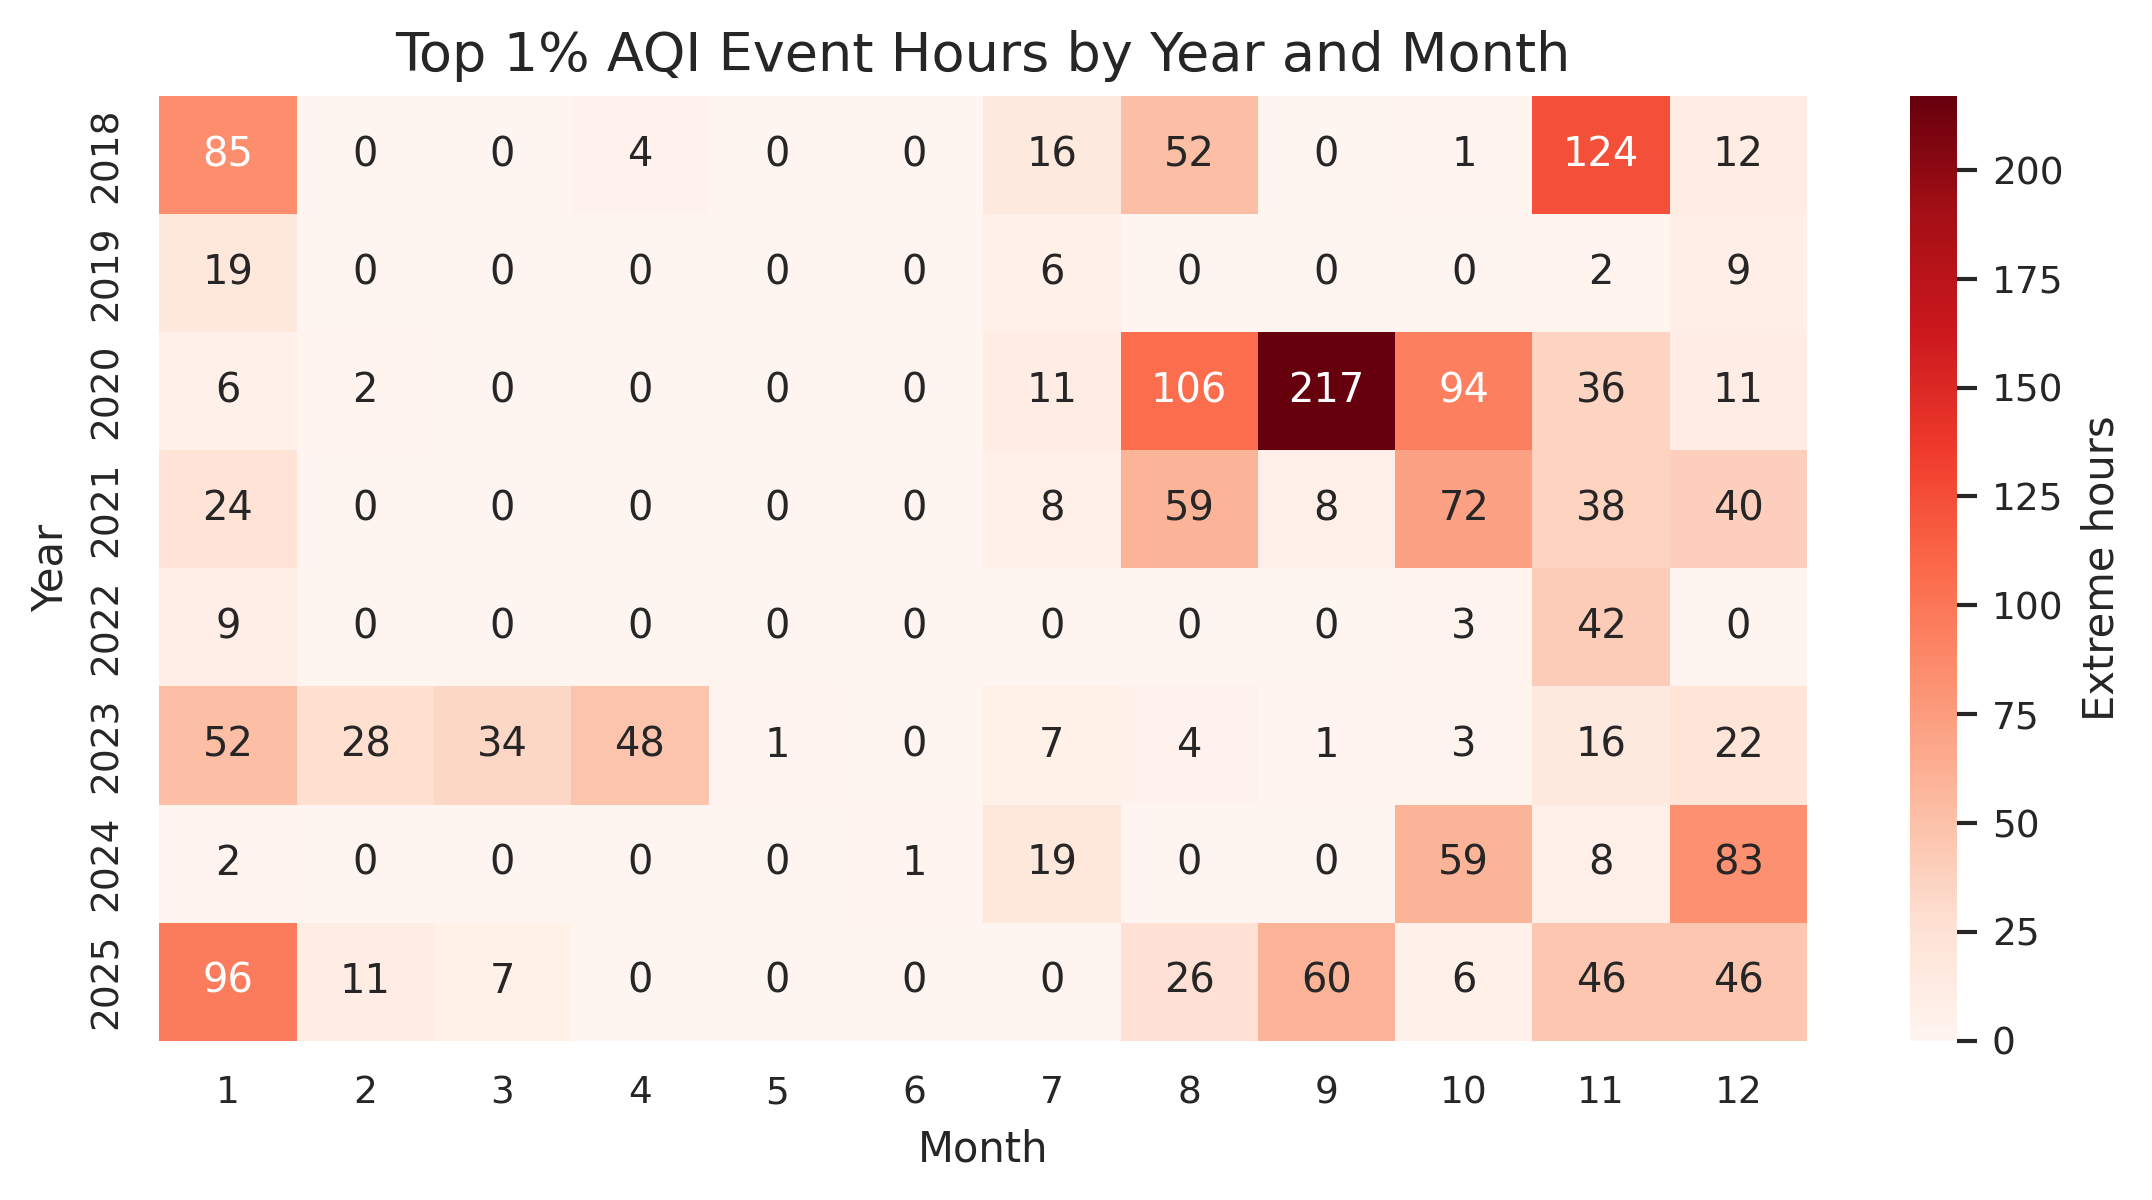
\includegraphics[width=0.82\linewidth]{figures/06_extreme_aqi_events_heatmap_year_month.png}
    \caption{Year-month heatmap of extreme AQI records (99th percentile threshold).}
    \label{fig:extreme-heatmap}
\end{figure}

Figure~\ref{fig:extreme-heatmap} shows strong temporal clustering during late summer and autumn, aligning with California wildfire seasons.

\section{Threats to Validity}\label{sec:threats}
Four main limitations apply. First, \texttt{target\_aqi} serves as a PM2.5 proxy rather than a full multi-pollutant AQI. Second, combining EPA AQS and Open-Meteo sources introduces potential data heterogeneity; 2025 relies predominantly on Open-Meteo records. Third, ablation reveals minimal standalone gain from VPD and spatial lags. Fourth, extreme-event clustering reflects correlation rather than causal fire attribution.

\section{Conclusion and Future Work}\label{sec:conclusion}
We presented a California AQI forecasting benchmark across 181,122 hourly records (2018--2025). XGBoost achieved top performance in short-term nowcasting ($R^2 = 0.8711$) and 24-hour forecasting ($R^2 = 0.4648$). However, scenario analysis shows machine learning models struggle during upper-tail spikes without real-time smoke transport inputs, where naive persistence baselines remain competitive.

Future work will incorporate satellite Aerosol Optical Depth (AOD), fire perimeters, planetary boundary layer height, and wind vector transport. We also plan to evaluate Spatio-Temporal Graph Neural Networks (ST-GNNs) for regional modeling and connect model outputs to automated IoT public health alerts.

\backmatter

\bmhead{Acknowledgements}
The authors acknowledge the U.S. Environmental Protection Agency for providing publicly accessible AQS monitoring data and Open-Meteo for supplemental meteorological records.

\section*{Declarations}
\begin{itemize}
\item \textbf{Funding}: Not applicable.
\item \textbf{Conflict of interest}: The authors declare no competing interests.
\item \textbf{Data availability}: The datasets generated and analysed during the current study are available from the EPA AQS and Open-Meteo public repositories.
\item \textbf{Code availability}: Code and reproducibility materials are available upon reasonable request.
\item \textbf{Author contribution}: All authors contributed to the study conception and design. Data collection, analysis, and implementation were performed by all authors. All authors read and approved the final manuscript.
\end{itemize}

\bibliography{references}

\end{document}
